\documentclass[8pt,t]{beamer}
\geometry{paperwidth=160mm,paperheight=0.75\paperwidth} % I can't make the fontsize smaller (than 8pt), but I can make the page bigger
\graphicspath{{figures/}} % Setting the graphicspath

% Theme settings
\usetheme{Madrid}
\usecolortheme{default}
\setbeamertemplate{navigation symbols}{}   % removes navigation symbols such as 'next page'
\setbeamertemplate{footline}{}             % remove line with name, date, page nr.
\setbeamercolor*{frametitle}{bg=white}     % remove background from frametitle
\usepackage{caption}
% \captionsetup[figure]{labelformat=empty}% redefines the caption setup of the figures environment in the beamer class.
\setbeamersize{text margin left=20pt,text margin right=10pt}
\usefonttheme[onlymath]{serif} % makes beamer math look like article math
\usepackage{hyperref}

%======================= title page info =======================
\title{The proton content at approximate N3LO accuracy}
\date{Milan Joint Phenomenology Seminar  \\[0.1cm] 6 June 2024}
\author{Roy Stegeman}
\institute{\small The University of Edinburgh}


%======================= page numbering =======================
\addtobeamertemplate{navigation symbols}{}{%
  \ifnum\thepage>1% don't display frame number on the first slide
    \usebeamerfont{footline}\insertframenumber\hspace*{2em}\vspace*{2em}% display frame number
  \fi%
}



%=================================== colors ====================================
\definecolor{RoyBlue}{RGB}{22, 46, 69}
\definecolor{RoyGrey}{RGB}{64, 88, 128}

\setbeamercolor{structure}{fg=RoyBlue} % itemize, enumerate, etc
\setbeamercolor{frametitle}{fg=RoyGrey}
\setbeamercolor{section in head/foot}{bg=RoyBlue}


%======================= add progress dots to headline =========================
% \setbeamertemplate{headline}{%
%     \begin{beamercolorbox}[ht=4mm,dp=4mm]{section in head/foot}
%         \insertnavigation{\paperwidth}
%     \end{beamercolorbox}%
% }%
% \makeatother


%======================= add section title page ================================
\newcommand{\SectionTitleFrame}[1][]{%
  \begin{frame}
    \vfill
    \centering
    \begin{beamercolorbox}[sep=8pt,center,shadow=true,rounded=true]{title}
      \usebeamerfont{title}\insertsection\par
    \end{beamercolorbox}
    % Include optional text if provided
    \ifx\relax#1\relax\else
      \vspace{0.5cm}
      \textbf{#1}
    \fi
    \vfill
  \end{frame}
}

% Use \SectionTitleFrame in \AtBeginSection
\AtBeginSection[]{
  \SectionTitleFrame
}


%=================================== titlepage =================================
\titlegraphic{\vspace*{6mm}
  
\includegraphics[height=1.5cm]{logos/edi_logo.png} \hspace{10mm}
  % 
\includegraphics[height=0.8cm]{logos/nnpdf_logo_official.pdf} \hspace{10mm}
  
\includegraphics[height=1.5cm]{logos/higgs_logo.jpg}
}

\defbeamertemplate{title page}{noinstitute}[1][]
{
  \vbox{}
  \vfill
  \begingroup
    \centering
    \begin{beamercolorbox}[sep=8pt,center,#1]{title}
      \usebeamerfont{title}\inserttitle\par%
      \ifx\insertsubtitle\@empty%
      \else%
        \vskip0.25em%
        {\usebeamerfont{subtitle}\usebeamercolor[fg]{subtitle}\insertsubtitle\par}%
      \fi%
    \end{beamercolorbox}%
    \vskip2em\par
    \begin{beamercolorbox}[sep=0pt,center,#1]{author}
      \usebeamerfont{author}\insertauthor
    \end{beamercolorbox}
  \begin{beamercolorbox}[sep=0pt,center,#1]{author}
    \usebeamerfont{institute}\insertinstitute
  \end{beamercolorbox}
  \vspace*{8pt}
  \vspace*{16pt}
    \begin{beamercolorbox}[sep=0pt,center,#1]{date}
      \usebeamerfont{date}\insertdate
    \end{beamercolorbox}\vskip0.5em
    {\usebeamercolor[fg]{titlegraphic}\inserttitlegraphic\par}
  \endgroup
  \vfill
}

\makeatletter
\setbeamertemplate{title page}[noinstitute][colsep=-4bp,rounded=true,shadow=\beamer@themerounded@shadow]
\makeatother


\begin{document}
{
\setbeamertemplate{headline}{} % remove headline from titlepage
\begin{frame}
  \titlepage
\end{frame}
}

\setbeamertemplate{enumerate items}[default]

\pgfdeclarelayer{bg}    % declare background layer
\pgfsetlayers{bg,main}  % set the order of the layers (main is the standard layer)



% Title: The proton content at N3LO accuracy

% Abstract: In recent years the accuracy of PDF determinations has significantly
% improved due to a combination of experimental and theoretical developments. In
% this talk, I will discuss recent progress towards the extension of the PDF
% determination to approximate N3LO in QCD and NLO in QED, and their
% phenomenological implications for a number of LHC processes. I will also
% present a simultaneous extraction of the strong coupling constant and the PDFs
% based on the NNPDF4.0 dataset, taking correlations between them into account.
% We show how we can validate our determination of the strong coupling by
% performing a closure test.

% SLIDES =======================================================================


\begin{frame}{Motivation: theoretical uncertainties at the LHC}
  % $$\sigma(x,Q^2)=\sum_i \int_x^1 \frac{dz}{z} \mathcal{L}_{ij}(z,\mu^2)\hat{\sigma}_{ij}\left(\frac{x}{z},\frac{Q^2}{\mu^2},\alpha_s\right)$$

  \begin{columns}
    \begin{column}{0.55\textwidth}
      The dominant uncertainties in theoretical predictions at the LHC are:
      \begin{itemize}
        \item Missing higher order uncertainties (from scale variations)
        \item PDF uncertainties
        \item Uncertainties on $\alpha_s$
      \end{itemize}

      \vspace*{0.5em}
      Progress towards improved theoretical accuracy:
      \begin{itemize}
        \item QED effects
        \item approximate N3LO
        \item Accounting for missing higher order uncertainties
        \item A simultaneous determination of the PDFs and $\alpha_s$
      \end{itemize}
    \end{column}
    \begin{column}{0.44\textwidth}
      \begin{figure}
        \centering
        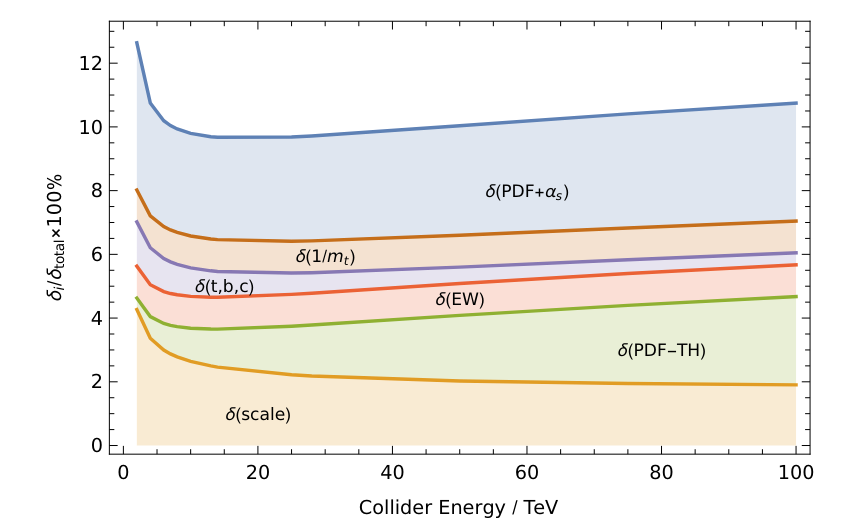
\includegraphics[width=0.8\textwidth]{figures/sources_of_unc_higgs.png}
        \caption*{ \small Uncertainties for inclusive Higgs production \\  {\color{gray}\footnotesize Dulat, Lazopoulos, Mistleberger, 1802.00827}}
      \end{figure}
    \end{column}
  \end{columns}
\end{frame}


\section*{approximate N3LO}
\SectionTitleFrame[\hyperlink{https://arxiv.org/abs/2402.18635}{arXiv: 2402.18635}]


\begin{frame}{What do we need for N3LO}
  % GLAP
  % Heavy flavor number scheme
  % DIS coeffs
  % Hadronic coeffs
\end{frame}

\begin{frame}{aN3LO splitting functions}
  % construct approximations from known results
  % show impact on evolution of gluon PDF
  % account for MHOUs and INHOUs
\end{frame}


\begin{frame}{N3LO corrections to DIS}
  % massive contributions can be approximated from known limits
  % extension of FONLL
\end{frame}

\begin{frame}{Inclusion of theory uncertainties}
  % covtot = covexp + covmhou + covihou
  % NNLO MHOU from ren scale var if N3LO not available
  % show chi2 as function of perturbative order plot
\end{frame}

\begin{frame}{Impact on LHC cross sections}
  % show the pheno plots for Higgs and DY
  % improve perturbative convergence
\end{frame}

\section*{QED}
\SectionTitleFrame[\hyperlink{https://arxiv.org/abs/2401.08749}{arXiv: 2401.08749}]


\begin{frame}{What is needed for a QED PDF set?}
  % Photon PDF for photon initiated states
    % modifies sum rule
  % NLO QED (and NNLO QCD) DGLAP running for radiatively generated photons
\end{frame}

\begin{frame}{Constructing the photon PDF}
  % data not very constraining so fit is not practical
  % compute from structure functions
    % structure functions obtained from pQCD and experiment
\end{frame}

\begin{frame}{Impact on LHC cross sections}
\end{frame}


\section*{$\alpha_s$ from NNPDF4.0}
\SectionTitleFrame[In preparation]

\begin{frame}{Propagating uncertainties in NNPDF}
  \begin{columns}
    \begin{column}{0.49\textwidth}
      Data is fully defined by central values $\mu_i$ and covariance matrix $\operatorname{cov}_{ij}$
      \begin{enumerate}
        \item Generate $N_{\rm rep}$ { Monte Carlo data} ``replicas'' $\hat{\mu}_i$ such that as $N_{\rm rep}\to \infty$ \\
        $\mu_i = \frac{1}{N_{\rm rep}}\sum_{i=1}^{N_{\rm rep}} \hat{\mu}_i$\\
        $\operatorname{cov}_{ij} = \operatorname{cov}[\hat{\mu}_i, \hat{\mu}_j]$
        \item Perform a { PDF fit} to each replica
        \item Compute observables $X$ and their uncertainties\\
        $\left\langle X\left[f\right]\right\rangle=\frac{1}{N_{\rm rep}} \sum_{r=1}^N X\left[f^{(r)}\right]$\\
        $\operatorname{Var}\left[X\left[f\right]\right] = \frac{1}{N_{\rm rep}} \sum_{r=1}^{N_{\rm rep}}\left(X\left[f^{(r)}\right]-\left\langle X\left[f\right]\right\rangle\right)^2$
      \end{enumerate}
    \end{column}
    \begin{column}{0.49\textwidth}
      \begin{center}
        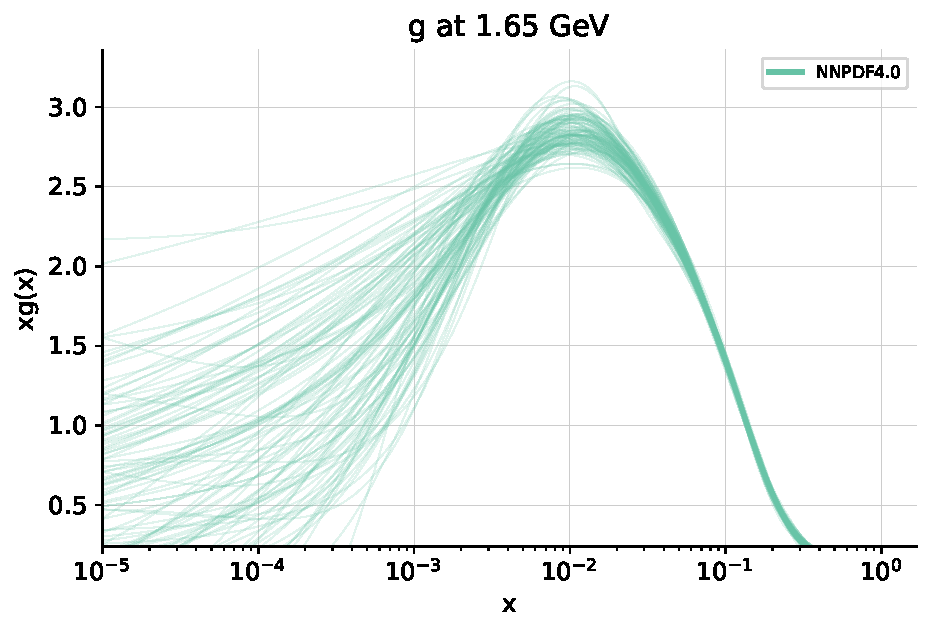
\includegraphics[width=0.7\textwidth]{replicas_g.pdf}\\
        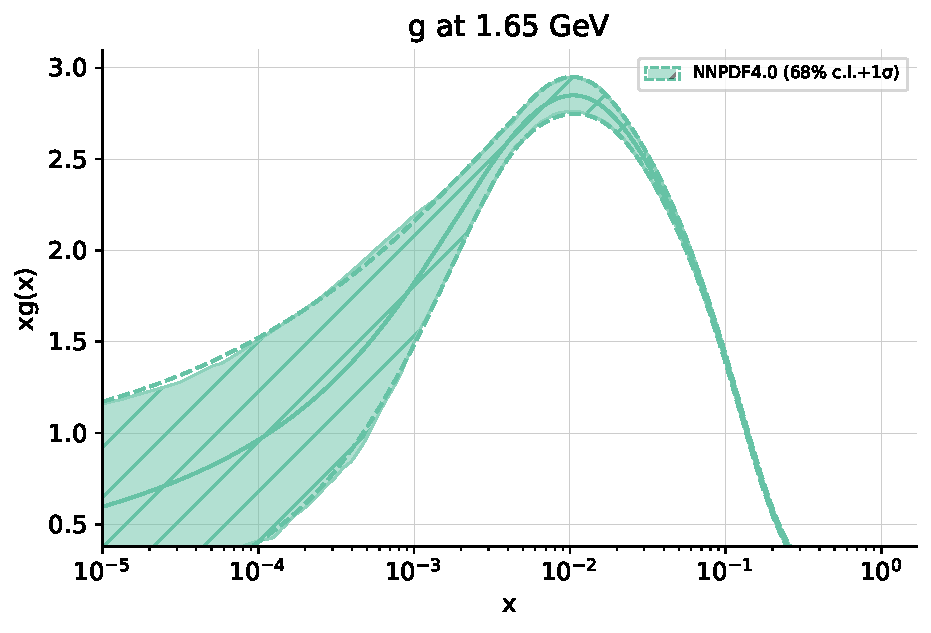
\includegraphics[width=0.7\textwidth]{band_g.pdf}
      \end{center}
    \end{column}
  \end{columns}
\end{frame}




\begin{frame}{Correlations between $\alpha_s$ and the PDFs}
  \begin{columns}[T]
    \begin{column}{0.49\textwidth}
      \begin{itemize}
        \item Usually $\alpha_s$ determination is done by repeating a PDF fit at different values of $\alpha_s$ and performing a parabolic fit
      \end{itemize}
    \end{column}
    \begin{column}{0.49\textwidth}
      \only<1>{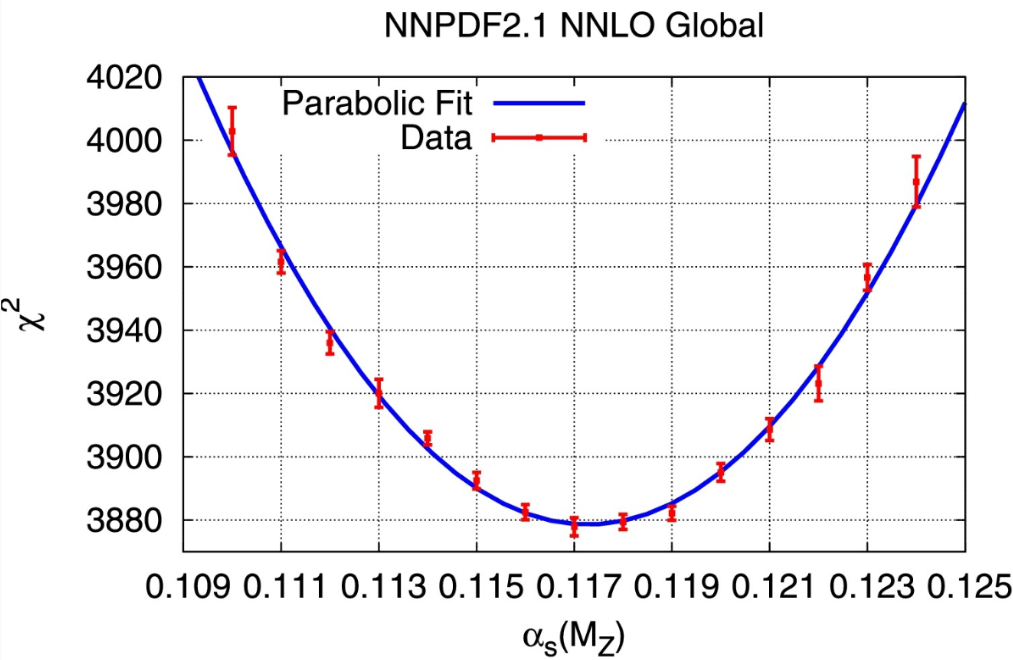
\includegraphics[width=0.7\textwidth]{exp_method.png}}
    \end{column}
  \end{columns}
  % cite Forte, Kassabov
  % explain usual methodology
  % explain correlated replicas method
\end{frame}

\begin{frame}{Correlations between $\alpha_s$ and the PDFs}
  \begin{columns}[T]
    \begin{column}{0.49\textwidth}
      \begin{itemize}
        \item Usually $\alpha_s$ determination is done by repeating a PDF fit at different values of $\alpha_s$ and performing a parabolic fit
        \item Such a determination misses correlations between $\alpha_s$ and the PDF parameters $\theta$, leading to \textbf{underestimated uncertainties}
      \end{itemize}
    \end{column}
    \begin{column}{0.49\textwidth}
      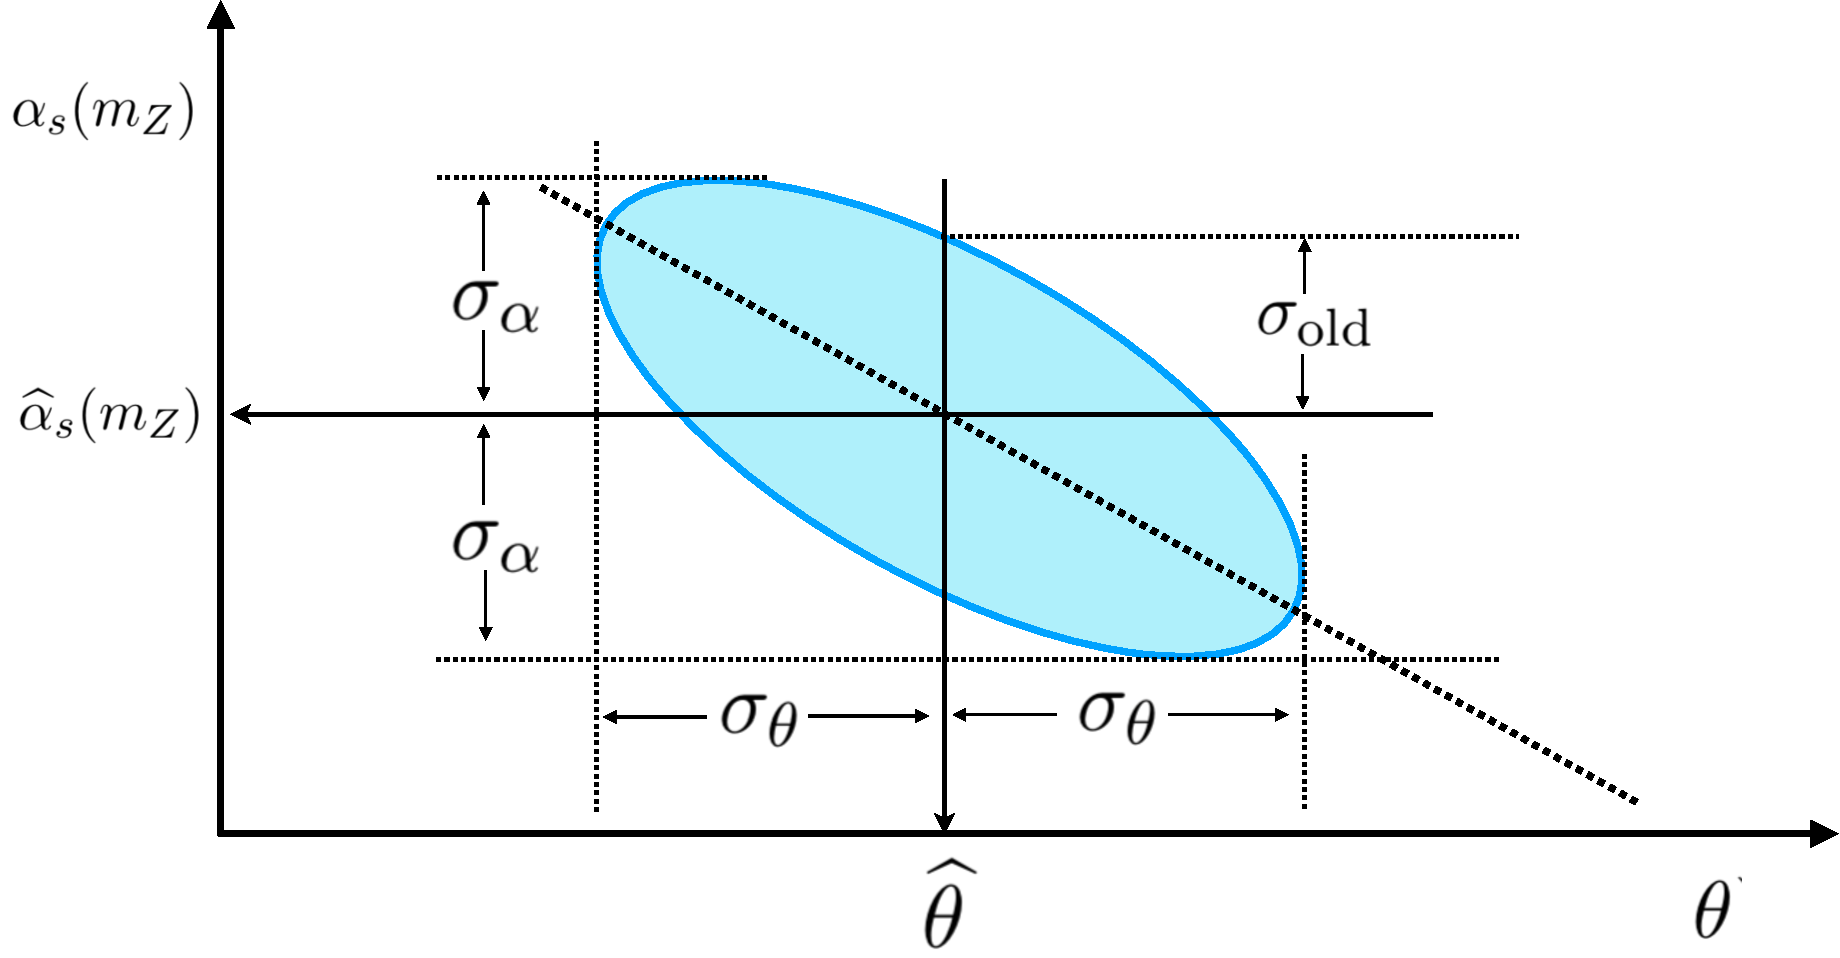
\includegraphics[width=0.9\textwidth]{ellipse.pdf}
    \end{column}
  \end{columns}
  % cite Forte, Kassabov
  % explain usual methodology
  % explain correlated replicas method
\end{frame}


\begin{frame}{A simultaneous optimization of $\alpha_s$}
  Ideally we would minimize simultaneously $\alpha_s$ and the PDF parameters but due to theories being stored in pre-computed grids at fixed values of $\alpha_s$ this is impractical

  % A simultaneous minimization implies solving the system of coupled equations
  % \begin{align}
  %   \label{eq:partial_theta}
  %   \frac{\partial}{\partial \theta} \chi^2(\alpha_s, \theta) &= 0 \\
  %   \frac{\partial}{\partial \alpha_s} \chi^2(\alpha_s, \theta) &= 0
  % \end{align}

  \vspace*{1em}

  A possible way to find the minimum in ($\alpha_s, \theta$) space is:
  \begin{enumerate}
    \item generate a set of pseudodata replicas
    \item fit these data replicas for different values of $\alpha_s$ (thus finding minima for $\theta$)
    \item for each replica, fit a parabola to get a $\chi^2(\alpha_s)$ profile
    \item each minimum corresponds to a sampled $\alpha_s$ value
  \end{enumerate}

\end{frame}


\begin{frame}{$\alpha_s$ from correlated theory uncertainties}

  In a PDF fit we minimize $\chi^2$:\\
  $P(T|D) \propto \exp\left[-\frac{1}{2}\left(T-D\right)^T\left(\mathrm{Cov}_\mathrm{exp}+\mathrm{Cov}_\mathrm{th}\right)^{-1}\left(T-D\right)\right]
  = \exp\left[-\frac{1}{2}\chi^2\right]$

  \vspace*{1em}
  We can model the theory uncertainty as a correlated shift: \\
  $T \rightarrow T + \lambda \beta $, \quad $\beta=\frac{\partial}{\partial \alpha_s}T$ (numerically, $\beta$ is constructed form discrete shifts)\\
  $P(T|D,\lambda) \propto \exp\left[-\frac{1}{2}\left(T+\lambda\beta-D\right)^T\left(\mathrm{Cov}_\mathrm{exp}+\mathrm{Cov}_\mathrm{th}\right)^{-1}\left(T+\lambda\beta-D\right)\right]$

  \vspace*{1em}
  We want to find $P(T|D)$ using Bayes' theorem, so we have to choose a prior for $\lambda$. Let us take a unit-width Gaussian\\
  $P(\lambda) \propto \exp\left[-\frac{1}{2}\lambda^2\right]$

  \vspace*{1em}
  Marginalizing over $\lambda$
  $P(T|D) \propto \int d\lambda \exp\left[Z^{-1}\left(\lambda-\bar{\lambda}\right)^2\right] $


  \vfill
  {\color{gray} \footnotesize Ball, Pearson, \hyperlink{https://arxiv.org/abs/2105.05114}{2105.05114}}
\end{frame}


\begin{frame}{How can we trust our methodology to correclty find $\alpha_s$?}
  Basic idea is that of a closure test:
  \begin{enumerate}
    \item generate data with theory predictions for a given value of $\alpha_s$
    \item see if the methodology correctly reproduces this known value
  \end{enumerate}

  More rigorous:
  % multiclosure test
\end{frame}


\begin{frame}{NNPDF4.0 results - preliminary}
  % Results with and without MHOU
\end{frame}



\appendix
\section{Backup}


\begin{frame}{Determination of the photon PDF}
  \begin{columns}[T]
    \begin{column}{0.59\textwidth}
      Initially the photon PDF has been determined in different ways:
      \begin{itemize}
        \item physical model: sensitive to underlying model
        \item fitting: data does not provide strong constraints
      \end{itemize}

      \vspace*{0.5em}
      However with the LUXqed approach it can be computed perturbatively \\
      based on the observation that the heavy-lepton production cross-section can be written in two ways:
      \begin{itemize}
        \item in terms of structure functions $F_2$, $F_L$
        \item in terms of PDFs (including the photon)
      \end{itemize}

      \vspace*{0.5em}
      luxQED result {\color{gray}\small[Manohar, Nason, Salam, Zanderighi: 1607.04266, 1708.01256]}:
      \vspace*{-0.8em}
      \begin{equation*}
        \begin{split}
          & x \gamma(x, \mu^2)
          =
          \frac{2}{\alpha (\mu^2)} \int\limits_x^1 \frac{dz}{z}
          \Biggl\{ \int_{m_p^2x^2 \over 1-z}^{\mu^2 \over 1-z} \frac{dQ^2}{Q^2}
          \alpha^2(Q^2) \Biggl[ -z^2 F_L(x/z, Q^2) \\
          & + \left( z P_{\gamma q}(z) + \frac{2 x^2 m_p^2}{Q^2} \right)
          F_2(x/z, Q^2)\Biggr] - \alpha^2(\mu^2) z^2 F_2(x/z, \mu^2)\Biggr\}
        \end{split}
      \end{equation*}
    \end{column}

    \begin{column}{0.39\textwidth}
      \vspace*{-2.5em}
      \begin{figure}
        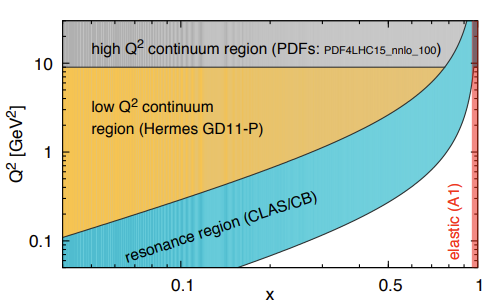
\includegraphics[width=0.89\textwidth]{figures/dataluxqed.png}
        \caption*{Input to construct $F_2$ and $F_L$}
        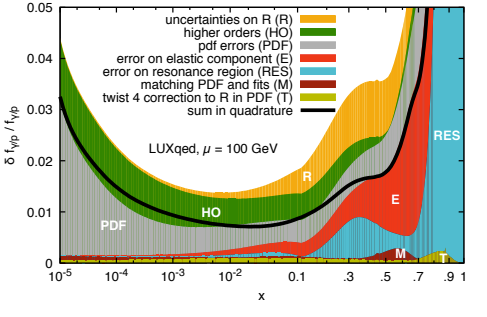
\includegraphics[width=0.89\textwidth]{figures/luxQED_uncs.png}
        \caption*{Sources of uncertainty}
      \end{figure}
    \end{column}
  \end{columns}
\end{frame}


\begin{frame}{LUXqed PDF determinations}
  LUXqed has been used in all of the most recent QED PDFs:
  \begin{itemize}
      \item LUXqed\_plus\_PDF4LHC15 {\color{gray}\small [1607.04266]}
      \item LUXqed17\_plus\_PDF4LHC15 {\color{gray}\small [1708.01256]}
      \item MMHT2015qed {\color{gray}\small [1907.02750]}
      \item NNPDF3.1luxQED {\color{gray}\small [1712.07053]}
      \item CT18lux and CT18qed {\color{gray}\small [2106.10299]}
      \item MSHT20QED {\color{gray}\small [2111.05357]}
      \item MSHT20qed\_an3lo {\color{gray}\small [2312.07665]}
      \item NNPDF4.0QED {\color{gray}\small [2401.08749 ]}
  \end{itemize}
\end{frame}

% \begin{frame}{Results: photon PDF and luminosity}
%   \begin{center}
%     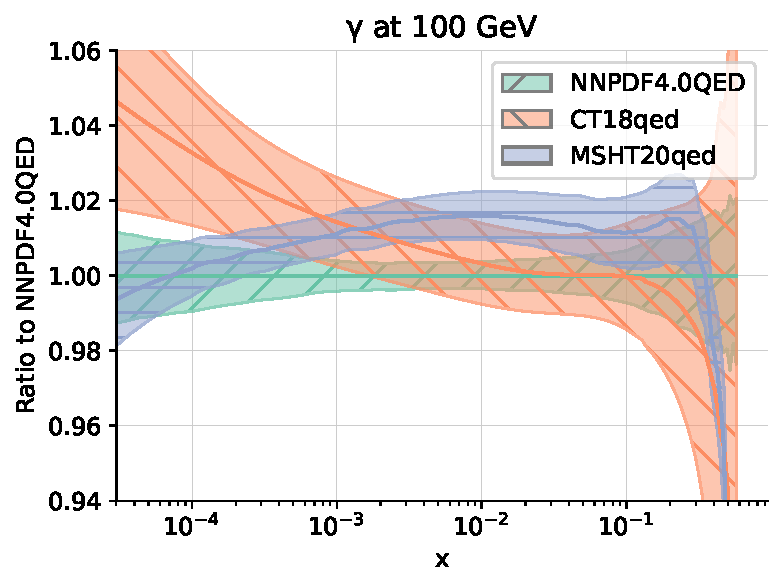
\includegraphics[width=0.3\textwidth]{figures/photon_comparison.pdf}
%     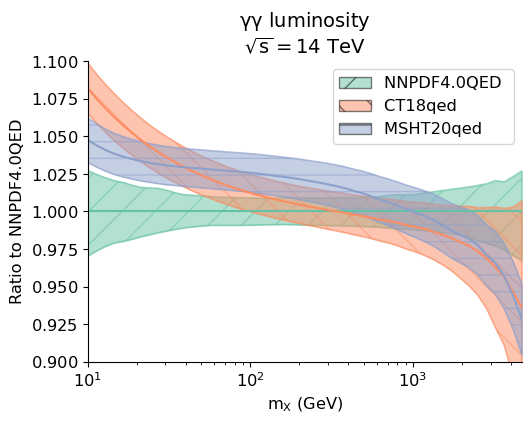
\includegraphics[width=0.3\textwidth]{figures/pp_lumi_comparison.png}
%     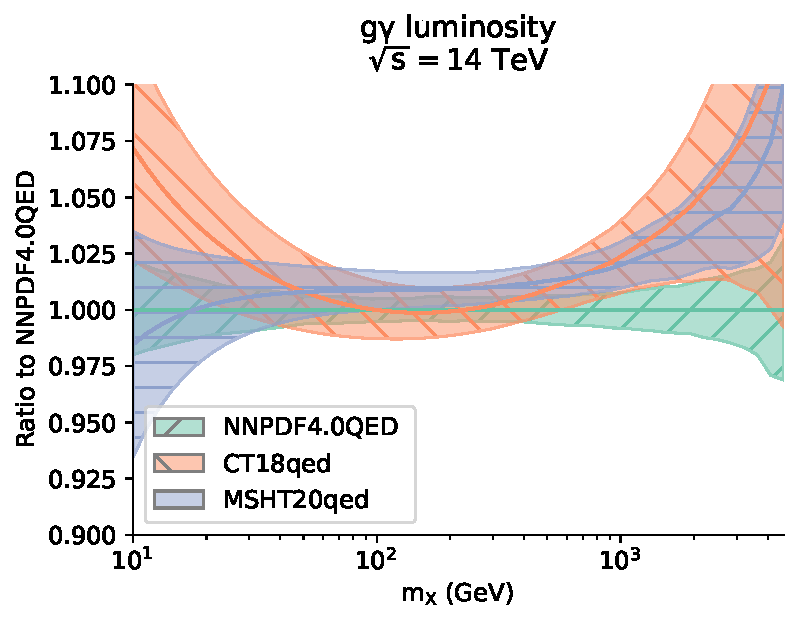
\includegraphics[width=0.3\textwidth]{figures/gp_lumi_comparison.pdf}
%   \end{center}
%   \begin{itemize}
%     \item Because all groups use the luxQED formalism, the photon PDFs agree at percent level
%     \item Luminosity generally in agreement, but differ at very small and very large invariant mass
%   \end{itemize}
% \end{frame}


% ============================================================================


\begin{frame}{Incomplete higher order uncertainties covmat}
  \begin{itemize}
    \item We construct an IHOU matrix following a similar approach by varying the subleading functions
    \item IHOU are independent of MHOU so the uncertainties are added in quadrature
    $$C = C_\mathrm{exp}+C_\mathrm{MHOU}+C_\mathrm{IHOU}$$
  \end{itemize}

  \begin{columns}
    \begin{column}{0.49\textwidth}
      \begin{figure}[!t]
        \centering
        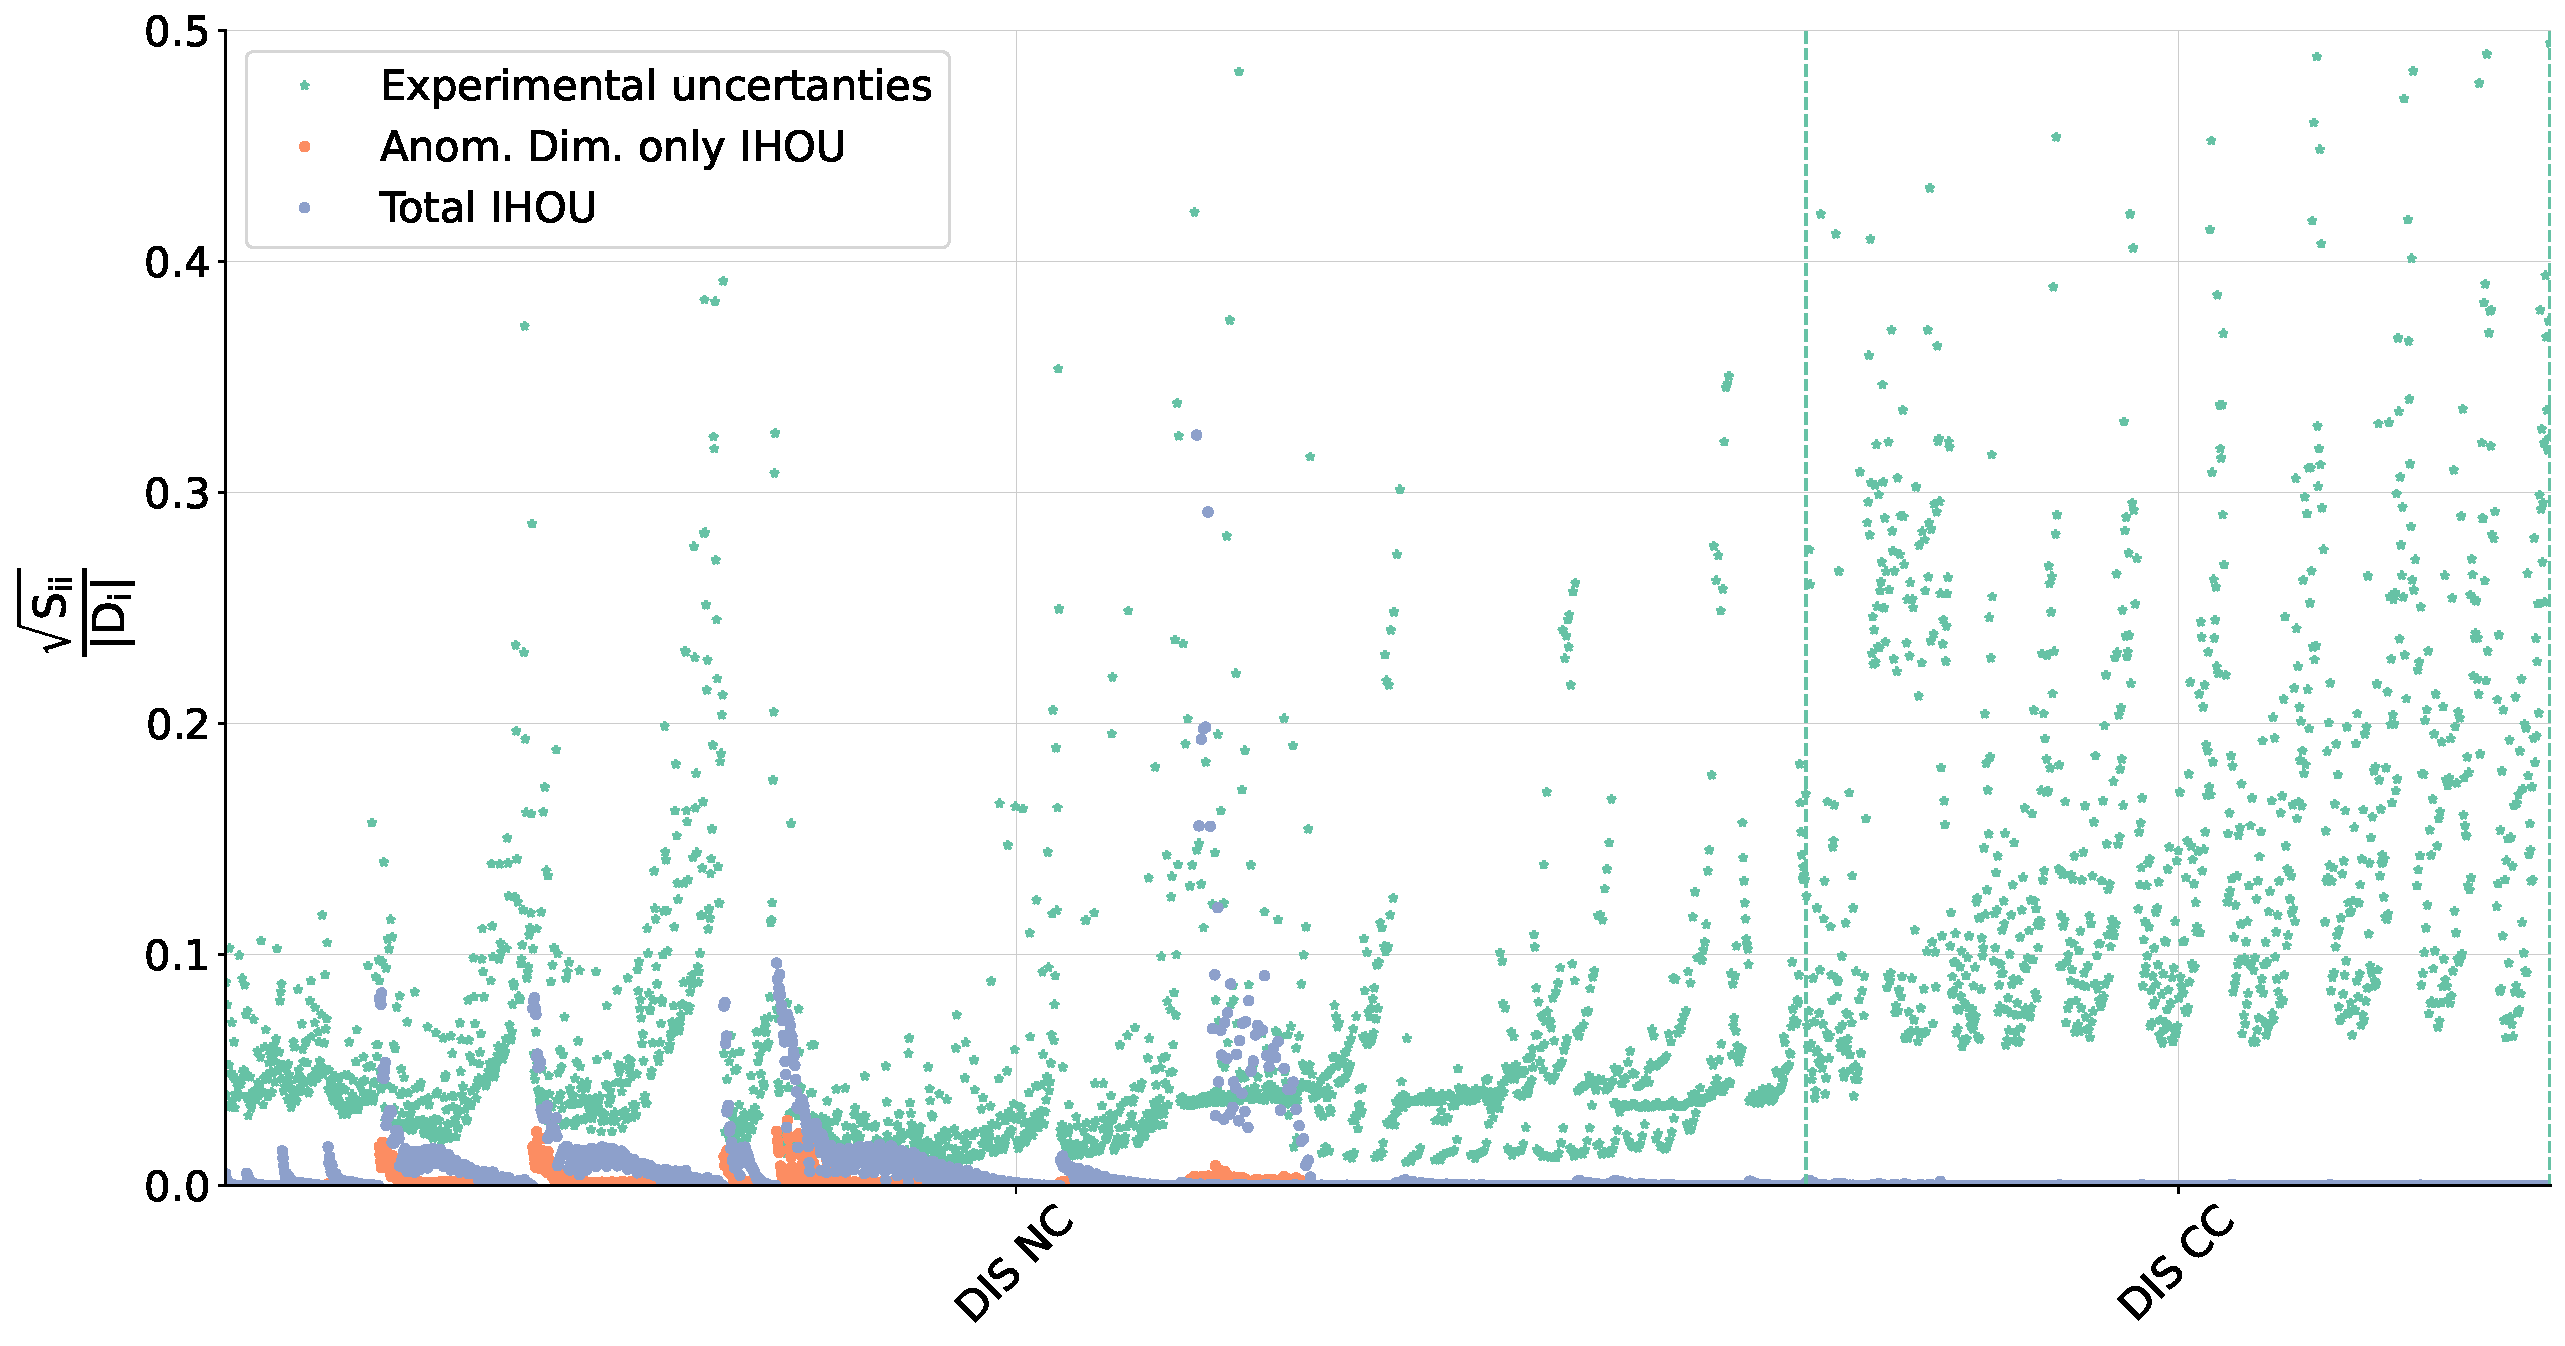
\includegraphics[width=.9\textwidth]{figures/diag_cov_dis_ihou.pdf}
        \caption*{IHOU have a large effect on small-$x$, low-$Q$ DIS data
        }
      \end{figure}
    \end{column}
    \begin{column}{0.49\textwidth}
      \begin{figure}[!t]
        \centering
        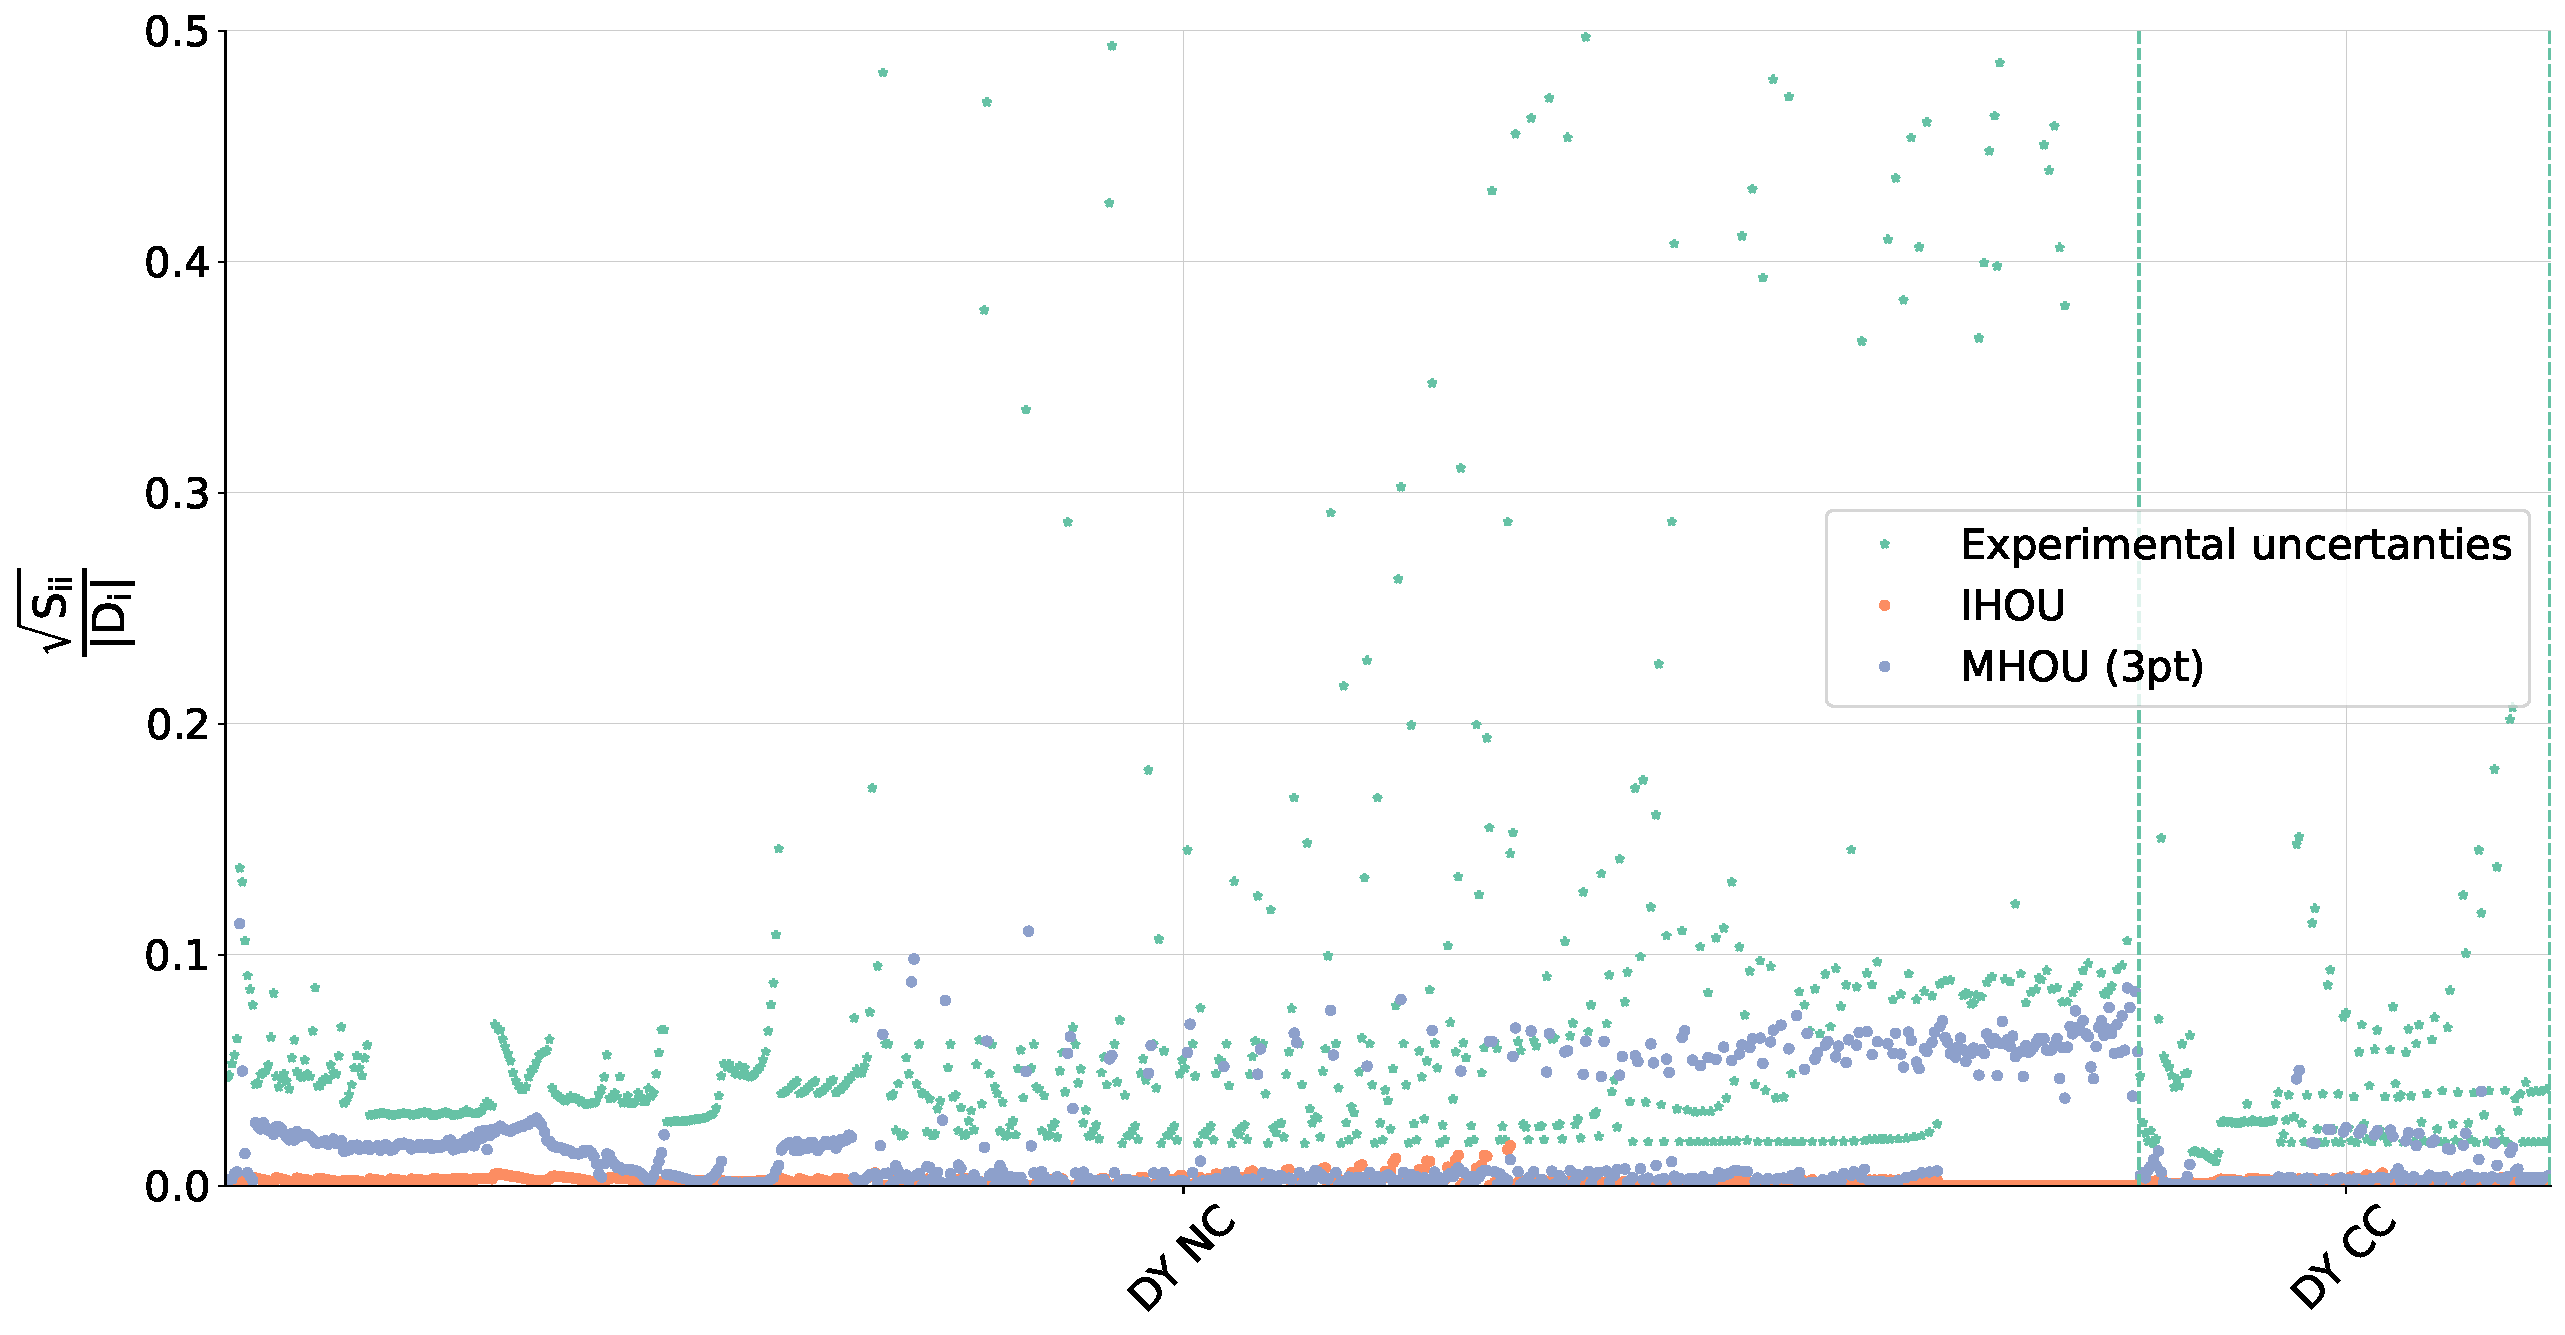
\includegraphics[width=.9\textwidth]{figures/diag_cov_dy_ihou_3pt_mhou.pdf}
        \caption*{NNLO MHOU included where N3LO not available \\
          MHOU can similar magnitude as the experimental uncertainty
        }
      \end{figure}
    \end{column}
  \end{columns}


\end{frame}

% \begin{frame}{Magnitude of theory uncertainties}
% % show that for certain processes th unc is of same size as exp unc.
% \end{frame}

% ============================================================================

\begin{frame}{Impact of MHOUs at N3LO}
  \begin{figure}[!t]
    \centering
    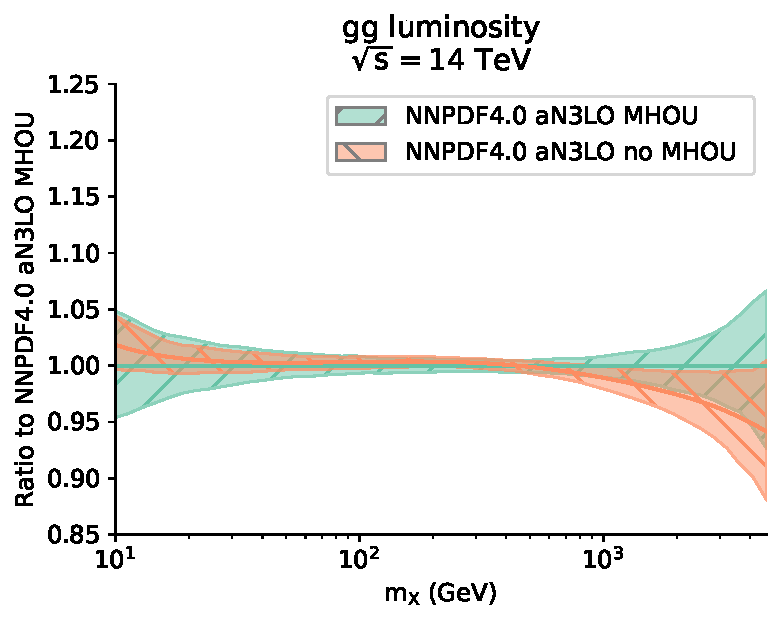
\includegraphics[width=0.45\textwidth]{figures/gg_plot_lumi1d.pdf}
    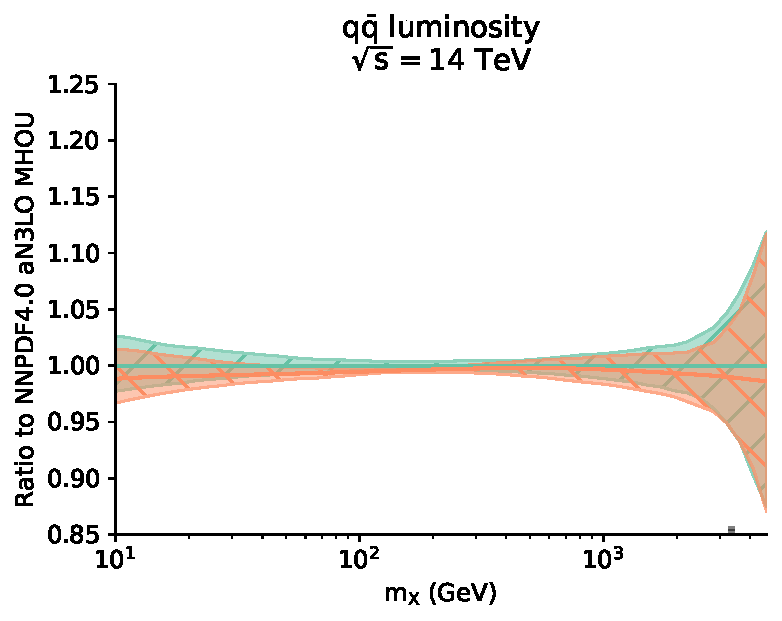
\includegraphics[width=0.45\textwidth]{figures/qqbar_plot_lumi1d.pdf}
  \end{figure}
  \begin{itemize}
    \item Non-negligible impact of MHOUs even at N3LO
    \item[$\Rightarrow$] reason to include exact N3LO calculations for hadronic processes
  \end{itemize}
\end{frame}


% \begin{frame}{Comparison to MSHT20}
%   \begin{figure}[!t]
%     \centering
%     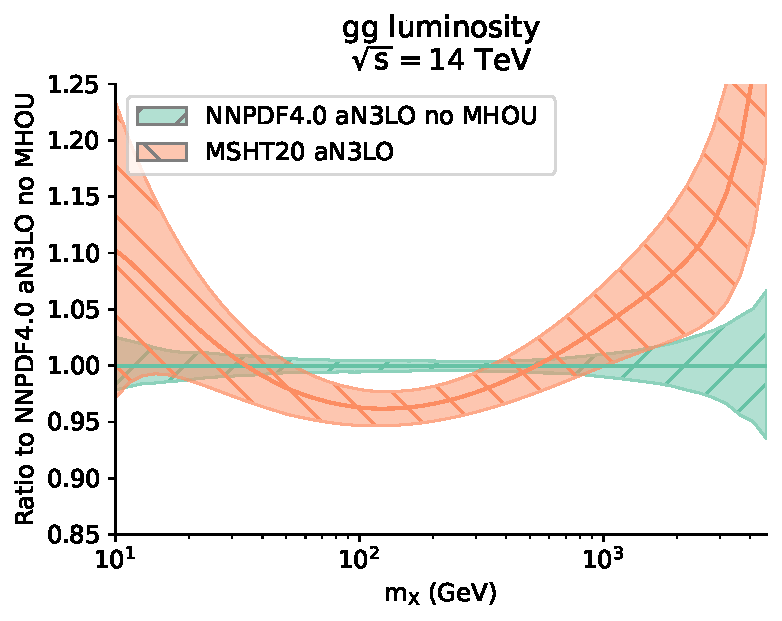
\includegraphics[width=0.45\textwidth]{figures/gg_plot_lumi1d_msht20.pdf}
%     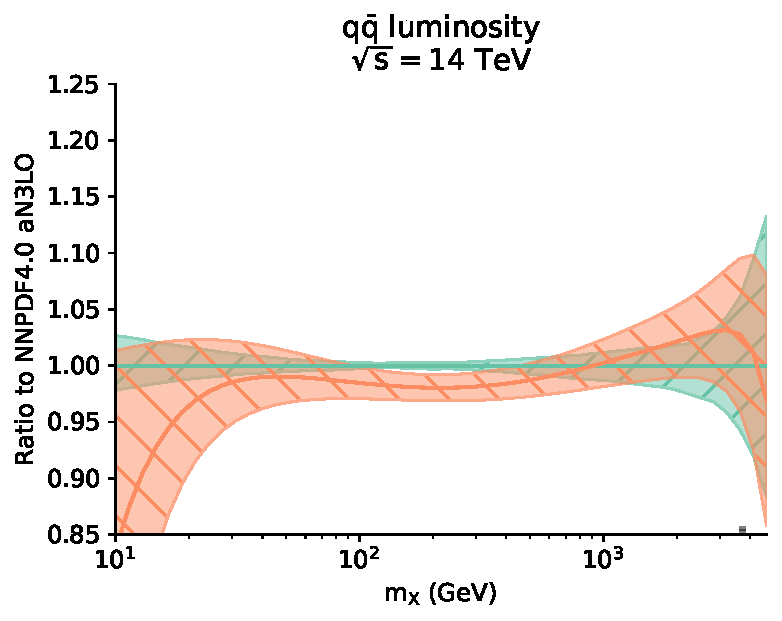
\includegraphics[width=0.45\textwidth]{figures/qqbar_plot_lumi1d_msht20.pdf}
%   \end{figure}
%   \begin{itemize}
%     \item Good agreement with MSHT20 for the quark luminosities
%     \item Also for gluon luminosities, except around the Higgs mass and high-mass
%     \item Similar data but different methodology (including splitting function parametrization)
%   \end{itemize}
% \end{frame}




\end{document}
